\begin{frame}{$\DPLL$ алгоритмы}

    \begin{center}
        \begin{frame}

    \begin{center}
        \Huge Part II: SAT Solving and Proof Complexity
    \end{center}
    
\end{frame}

\begin{frame}{$\DPLL$ Algorithms}

    \begin{center}
        \begin{frame}

    \begin{center}
        \Huge Part II: SAT Solving and Proof Complexity
    \end{center}
    
\end{frame}

\begin{frame}{$\DPLL$ Algorithms}

    \begin{center}
        \begin{frame}

    \begin{center}
        \Huge Part II: SAT Solving and Proof Complexity
    \end{center}
    
\end{frame}

\begin{frame}{$\DPLL$ Algorithms}

    \begin{center}
        \input{pics/dpll.tex}        
    \end{center}

    
	\pause
    \pause
    \pause
    \pause
    \pause
    \begin{itemize}
        \item Heuristic $\mathbf{A}$ chooses a variable for splitting.
    	\pause
	    \item Heuristic $\mathbf{B}$ chooses the first value.
    	\pause
    	\item Simplification rules: \alert{no simplifications!}
    \end{itemize}
\end{frame}

\begin{frame}{$\DPLL$ and Resolution}
    
    \begin{theorem}
        $\DPLL$ algoritm makes $t$ splitting on \alert{unsatisfiable} CNF formula
        $$\varphi \coloneqq \bigwedge\limits_i C_i$$
        $\Rightarrow$ there exists a resolution proof of $\varphi$ of size $2t$.
    \end{theorem}

    \pause

    \begin{minipage}{0.58\linewidth}
        \centering
        \input{pics/dpll-2.tex}
    \end{minipage}
    \pause
    \begin{minipage}{0.4\linewidth}
        \centering
        $\frac{A \lor x ~~~ B \lor \neg x}{A \lor B} ~~~~~ \frac{A}{A \lor z}$
        \begin{itemize}
            \item Node $\Rightarrow$ disjunction of negations of queries.
            \item $(x \lor \neg y \lor \neg z \lor u)$.
        \end{itemize}
    \end{minipage}

\end{frame}

\begin{frame}{Corollaries}

    \begin{itemize}
        \item{} Running time of $\DPLL$ on $\PHP_{n}^{n + 1}$ is at least $2^{\Omega(n)}$.
            \pause
        \item{} [Alekhnovich, Hirsch, Itsykson 05; \alert{informal}] Running time of \alert{restricted}
            $\DPLL$ on some \alert{sat. formulas} is at least $2^{\Omega(n)}$. 
    \end{itemize}

    \pause
    \vspace{0.5cm}
    \begin{block}{Remark}
        $\alg{CDCL} \approx$ general resolution.
    \end{block}

    \pause
    \begin{itemize}
        \item{} Running time of $\alg{CDCL}$ on $\PHP_{n}^{n + 1}$ is at least $2^{\Omega(n)}$.
        \item{} \alert{Open problem}: what about sat. formulas and $\alg{CDCL}$?
    \end{itemize}

\end{frame}
        
    \end{center}

    
	\pause
    \pause
    \pause
    \pause
    \pause
    \begin{itemize}
        \item Heuristic $\mathbf{A}$ chooses a variable for splitting.
    	\pause
	    \item Heuristic $\mathbf{B}$ chooses the first value.
    	\pause
    	\item Simplification rules: \alert{no simplifications!}
    \end{itemize}
\end{frame}

\begin{frame}{$\DPLL$ and Resolution}
    
    \begin{theorem}
        $\DPLL$ algoritm makes $t$ splitting on \alert{unsatisfiable} CNF formula
        $$\varphi \coloneqq \bigwedge\limits_i C_i$$
        $\Rightarrow$ there exists a resolution proof of $\varphi$ of size $2t$.
    \end{theorem}

    \pause

    \begin{minipage}{0.58\linewidth}
        \centering
        \tikzstyle{inner} = [circle, minimum size = 0.3cm, draw, inner sep = 0.1pt]
\tikzstyle{gstyle} = [fill = green]
\tikzstyle{rstyle} = [fill = red]
\tikzstyle{ed} = [->, draw]
\tikzstyle{ops} = [alt=<{#1-}>{opacity = 1}{opacity = 0}]
\tikzstyle{opstyle} = [inner, ops = #1]
\tikzstyle{oped} = [ed, ops = #1]
\tikzstyle{gstyle} = [alt=<{#1}>{fill = green}{}]
\tikzstyle{rstyle} = [alt=<{#1}>{red!90!black}{}]
\tikzstyle{snakestyle} = [
    alt=<{#1}>{
        decorate,
        decoration = {
            snake,
            amplitude = 0.4mm,
            segment length = 2mm,
            post length = 1mm
        }
    }{}]


    
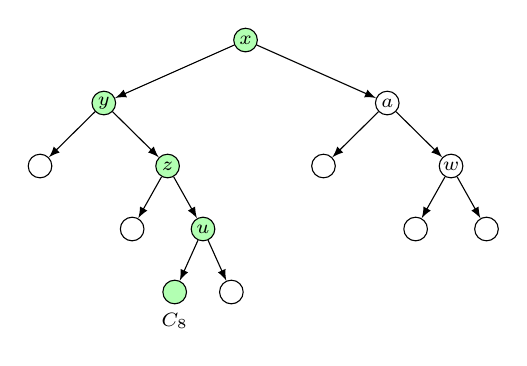
\begin{tikzpicture}[>=latex, xscale = 0.9]
    
    \node[inner, fill = green!30] (a) at (0, 0) {\scriptsize $x$};
    \node[inner, fill = green!30] (b) at (-2, -0.8) {\scriptsize $y$};
    \node[inner] (c) at (2, -0.8) {\scriptsize $a$};
    \node[inner] (d) at (-2.9, -1.6) {};
    \node[inner, fill = green!30] (e) at (-1.1, -1.6) {\scriptsize $z$};
    \node[inner] (f) at (1.1, -1.6) {};
    \node[inner] (g) at (2.9, -1.6) {\scriptsize $w$};

    \node[inner] (h) at (-1.6, -2.4) {};
	\node[inner, fill = green!30] (i) at (-0.6, -2.4) {\scriptsize $u$};
    
    \node[inner] (j) at (2.4, -2.4) {};
    \node[inner] (k) at (3.4, -2.4) {};

    \node[inner, fill = green!30] (l) at (-1, -3.2) {};
    \node[below = 4pt] at (l) {\scriptsize $C_{8}$};
    \node[inner] (m) at (-0.2, -3.2) {};
    
    \draw[ed] (a) -- (b);
    \draw[ed] (a) -- (c);
    \draw[ed] (b) -- (d);
    \draw[ed] (b) -- (e);
    \draw[ed] (c) -- (f);
    \draw[ed] (c) -- (g);
    \draw[ed] (e) -- (h);
    \draw[ed] (e) -- (i);
    \draw[ed] (g) -- (j);
    \draw[ed] (g) -- (k);
    \draw[ed] (i) -- (l);
    \draw[ed] (i) -- (m);
\end{tikzpicture}
    \end{minipage}
    \pause
    \begin{minipage}{0.4\linewidth}
        \centering
        $\frac{A \lor x ~~~ B \lor \neg x}{A \lor B} ~~~~~ \frac{A}{A \lor z}$
        \begin{itemize}
            \item Node $\Rightarrow$ disjunction of negations of queries.
            \item $(x \lor \neg y \lor \neg z \lor u)$.
        \end{itemize}
    \end{minipage}

\end{frame}

\begin{frame}{Corollaries}

    \begin{itemize}
        \item{} Running time of $\DPLL$ on $\PHP_{n}^{n + 1}$ is at least $2^{\Omega(n)}$.
            \pause
        \item{} [Alekhnovich, Hirsch, Itsykson 05; \alert{informal}] Running time of \alert{restricted}
            $\DPLL$ on some \alert{sat. formulas} is at least $2^{\Omega(n)}$. 
    \end{itemize}

    \pause
    \vspace{0.5cm}
    \begin{block}{Remark}
        $\alg{CDCL} \approx$ general resolution.
    \end{block}

    \pause
    \begin{itemize}
        \item{} Running time of $\alg{CDCL}$ on $\PHP_{n}^{n + 1}$ is at least $2^{\Omega(n)}$.
        \item{} \alert{Open problem}: what about sat. formulas and $\alg{CDCL}$?
    \end{itemize}

\end{frame}
        
    \end{center}

    
	\pause
    \pause
    \pause
    \pause
    \pause
    \begin{itemize}
        \item Heuristic $\mathbf{A}$ chooses a variable for splitting.
    	\pause
	    \item Heuristic $\mathbf{B}$ chooses the first value.
    	\pause
    	\item Simplification rules: \alert{no simplifications!}
    \end{itemize}
\end{frame}

\begin{frame}{$\DPLL$ and Resolution}
    
    \begin{theorem}
        $\DPLL$ algoritm makes $t$ splitting on \alert{unsatisfiable} CNF formula
        $$\varphi \coloneqq \bigwedge\limits_i C_i$$
        $\Rightarrow$ there exists a resolution proof of $\varphi$ of size $2t$.
    \end{theorem}

    \pause

    \begin{minipage}{0.58\linewidth}
        \centering
        \tikzstyle{inner} = [circle, minimum size = 0.3cm, draw, inner sep = 0.1pt]
\tikzstyle{gstyle} = [fill = green]
\tikzstyle{rstyle} = [fill = red]
\tikzstyle{ed} = [->, draw]
\tikzstyle{ops} = [alt=<{#1-}>{opacity = 1}{opacity = 0}]
\tikzstyle{opstyle} = [inner, ops = #1]
\tikzstyle{oped} = [ed, ops = #1]
\tikzstyle{gstyle} = [alt=<{#1}>{fill = green}{}]
\tikzstyle{rstyle} = [alt=<{#1}>{red!90!black}{}]
\tikzstyle{snakestyle} = [
    alt=<{#1}>{
        decorate,
        decoration = {
            snake,
            amplitude = 0.4mm,
            segment length = 2mm,
            post length = 1mm
        }
    }{}]


    
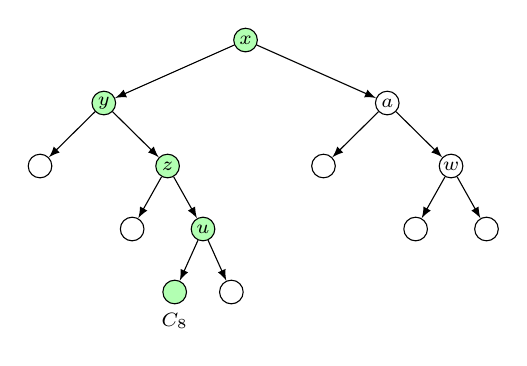
\begin{tikzpicture}[>=latex, xscale = 0.9]
    
    \node[inner, fill = green!30] (a) at (0, 0) {\scriptsize $x$};
    \node[inner, fill = green!30] (b) at (-2, -0.8) {\scriptsize $y$};
    \node[inner] (c) at (2, -0.8) {\scriptsize $a$};
    \node[inner] (d) at (-2.9, -1.6) {};
    \node[inner, fill = green!30] (e) at (-1.1, -1.6) {\scriptsize $z$};
    \node[inner] (f) at (1.1, -1.6) {};
    \node[inner] (g) at (2.9, -1.6) {\scriptsize $w$};

    \node[inner] (h) at (-1.6, -2.4) {};
	\node[inner, fill = green!30] (i) at (-0.6, -2.4) {\scriptsize $u$};
    
    \node[inner] (j) at (2.4, -2.4) {};
    \node[inner] (k) at (3.4, -2.4) {};

    \node[inner, fill = green!30] (l) at (-1, -3.2) {};
    \node[below = 4pt] at (l) {\scriptsize $C_{8}$};
    \node[inner] (m) at (-0.2, -3.2) {};
    
    \draw[ed] (a) -- (b);
    \draw[ed] (a) -- (c);
    \draw[ed] (b) -- (d);
    \draw[ed] (b) -- (e);
    \draw[ed] (c) -- (f);
    \draw[ed] (c) -- (g);
    \draw[ed] (e) -- (h);
    \draw[ed] (e) -- (i);
    \draw[ed] (g) -- (j);
    \draw[ed] (g) -- (k);
    \draw[ed] (i) -- (l);
    \draw[ed] (i) -- (m);
\end{tikzpicture}
    \end{minipage}
    \pause
    \begin{minipage}{0.4\linewidth}
        \centering
        $\frac{A \lor x ~~~ B \lor \neg x}{A \lor B} ~~~~~ \frac{A}{A \lor z}$
        \begin{itemize}
            \item Node $\Rightarrow$ disjunction of negations of queries.
            \item $(x \lor \neg y \lor \neg z \lor u)$.
        \end{itemize}
    \end{minipage}

\end{frame}

\begin{frame}{Corollaries}

    \begin{itemize}
        \item{} Running time of $\DPLL$ on $\PHP_{n}^{n + 1}$ is at least $2^{\Omega(n)}$.
            \pause
        \item{} [Alekhnovich, Hirsch, Itsykson 05; \alert{informal}] Running time of \alert{restricted}
            $\DPLL$ on some \alert{sat. formulas} is at least $2^{\Omega(n)}$. 
    \end{itemize}

    \pause
    \vspace{0.5cm}
    \begin{block}{Remark}
        $\alg{CDCL} \approx$ general resolution.
    \end{block}

    \pause
    \begin{itemize}
        \item{} Running time of $\alg{CDCL}$ on $\PHP_{n}^{n + 1}$ is at least $2^{\Omega(n)}$.
        \item{} \alert{Open problem}: what about sat. formulas and $\alg{CDCL}$?
    \end{itemize}

\end{frame}
        
    \end{center}

    
	\pause
    \pause
    \pause
    \pause
    \pause
    \begin{itemize}
        \item Эвристика $\mathbf{A}$ выбирает переменную для расщепления.
    	\pause
	    \item Эвристика $\mathbf{B}$ выбирает значения.
    	\pause
    	\item Правила упрощения: \alert{предположим, что их нет}.
    \end{itemize}
\end{frame}

\begin{frame}{$\DPLL$ и резолюция}
    
    \begin{theorem}
        $\DPLL$ алгоритм делает $t$ расщеплений на невыполнимой формуле
        $$\varphi \coloneqq \bigvee\limits_i C_i$$
        $\Rightarrow$ существует резолюционное доказательство $\varphi$ размера $2t$.
    \end{theorem}

    \pause

    \begin{minipage}{0.58\linewidth}
        \centering
        \tikzstyle{inner} = [circle, minimum size = 0.3cm, draw, inner sep = 0.1pt]
\tikzstyle{gstyle} = [fill = green]
\tikzstyle{rstyle} = [fill = red]
\tikzstyle{ed} = [->, draw]
\tikzstyle{ops} = [alt=<{#1-}>{opacity = 1}{opacity = 0}]
\tikzstyle{opstyle} = [inner, ops = #1]
\tikzstyle{oped} = [ed, ops = #1]
\tikzstyle{gstyle} = [alt=<{#1}>{fill = green}{}]
\tikzstyle{rstyle} = [alt=<{#1}>{red!90!black}{}]
\tikzstyle{snakestyle} = [
    alt=<{#1}>{
        decorate,
        decoration = {
            snake,
            amplitude = 0.4mm,
            segment length = 2mm,
            post length = 1mm
        }
    }{}]


    
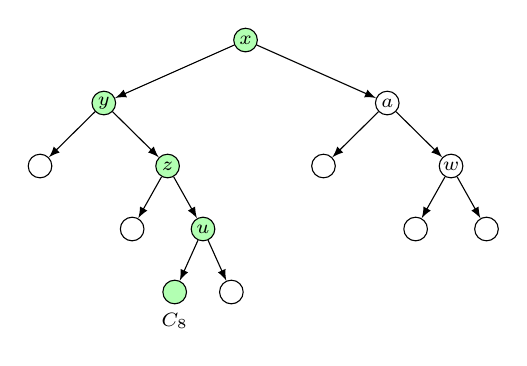
\begin{tikzpicture}[>=latex, xscale = 0.9]
    
    \node[inner, fill = green!30] (a) at (0, 0) {\scriptsize $x$};
    \node[inner, fill = green!30] (b) at (-2, -0.8) {\scriptsize $y$};
    \node[inner] (c) at (2, -0.8) {\scriptsize $a$};
    \node[inner] (d) at (-2.9, -1.6) {};
    \node[inner, fill = green!30] (e) at (-1.1, -1.6) {\scriptsize $z$};
    \node[inner] (f) at (1.1, -1.6) {};
    \node[inner] (g) at (2.9, -1.6) {\scriptsize $w$};

    \node[inner] (h) at (-1.6, -2.4) {};
	\node[inner, fill = green!30] (i) at (-0.6, -2.4) {\scriptsize $u$};
    
    \node[inner] (j) at (2.4, -2.4) {};
    \node[inner] (k) at (3.4, -2.4) {};

    \node[inner, fill = green!30] (l) at (-1, -3.2) {};
    \node[below = 4pt] at (l) {\scriptsize $C_{8}$};
    \node[inner] (m) at (-0.2, -3.2) {};
    
    \draw[ed] (a) -- (b);
    \draw[ed] (a) -- (c);
    \draw[ed] (b) -- (d);
    \draw[ed] (b) -- (e);
    \draw[ed] (c) -- (f);
    \draw[ed] (c) -- (g);
    \draw[ed] (e) -- (h);
    \draw[ed] (e) -- (i);
    \draw[ed] (g) -- (j);
    \draw[ed] (g) -- (k);
    \draw[ed] (i) -- (l);
    \draw[ed] (i) -- (m);
\end{tikzpicture}
    \end{minipage}
    \pause
    \begin{minipage}{0.4\linewidth}
        \centering
        $\frac{A \lor x ~~~ B \lor \neg x}{A \lor B} ~~~~~ \frac{A}{A \lor z}$
        \begin{itemize}
            \item Вершина $\Rightarrow$ дизъюнкция отрациний запросов.
            \item $(x \lor \neg y \lor \neg z \lor u)$.
        \end{itemize}
    \end{minipage}

\end{frame}


\begin{frame}{Следствия}

    \begin{itemize}
        \item{} [Следствие из Haken 85] $\DPLL$ алгоритмы будут работать не менее $2^{\Omega(n)}$ шагов
            на формулах $\PHP_{n}^{n + 1}$.
            \pause
        \item{} [Алехнович, Гирш, Ицыксон 05; \alert{неформально}] На выполнимых формулах
            <<ограниченные>> $\DPLL$ алгоритмы требуют экспоненциального времени.
            \pause
        \item{} [Ицыксон, C 11; \alert{неформально}] <<В среднем>> на выполнимых формулах
            <<ограниченные>> $\DPLL$ алгоритмы требуют экспоненциального времени.
    \end{itemize}

\end{frame}
